\documentclass[10pt]{article}
\usepackage{listings}
\usepackage{graphicx}
\usepackage{url}

% global commands

\newcommand{\javalst}[2]{
  \lstset{language=Java,captionpos=b,tabsize=4,frame=single,numbers=left,
    numberstyle=\tiny,numbersep=10pt,breaklines=true,showstringspaces=false,
    basicstyle=\footnotesize,emph={label}, caption={#1}, label={#2}}
}
\newcommand{\initlisting}[2]{
  \lstset{language={#1},captionpos=b,tabsize=4,frame=single,numbers=left,
    numberstyle=\tiny,numbersep=10pt,breaklines=true,showstringspaces=false,
    basicstyle=\footnotesize,emph={label}, caption={#2}}
}

\newcommand{\nm}{{\bf proTrade}}
\newcommand{\nmsp}{{\nm \ }}
% end commands
\setlength{\parskip}{0.3cm}
\setlength{\parindent}{0cm}

\begin{document}

\title{Report Three: Software Validation}

\author{Corina Ciobanu \and Iskander Orazbekov \and Mir Sahin \and Paul Grigoras \and Radu Baltean-Lugojan}

\date{\today}         % inserts today's date

\maketitle            % generates the title from the data above

\begin{abstract}
  \nmsp is a tennis trading environment which delivers the information a trader requires to place bets. Betting functionality, linked to the user's bank account is also provided. Testing and validation are crucial in order to deliver a reliable and secure application and have been used extensively.
\end{abstract}

\tableofcontents


\section{Introduction}
Tennis trading is a steadily growing market on the Betfair Exchange, with more than 70\% of bets being placed in-play. In order to maintain market liquidity, exchanges must attract customers. One way to achieve this is to provide the users with better tools which, by providing more information and better visualization techniques, can help the trader improve his understanding and predict the market evolution, ultimately leading to an increase in his profit.

In the case of tennis trading, the information required to understand and predict the evolution of the market associated with a particular match consists of the live score, player statistics, potentially a live video feed and - of course - the market data (evolution of betting odds). Ideally, this information is desired for both historical and live matches.

At the moment, no application provides all this information. A number of solutions exist which allow visualization of historical market data, but they generally lack the more specific, tennis related data. For example the Fracsoft Data Viewer (\cite{site-fracsoft}) does not correlate market data with match data (scores, player statistics). BetAngel (\cite{site-betangel}) provides some tennis related data and prediction, but relies on the user to input the current match score by pushing buttons. This not entirely suited for the high rate at which data is updated. Ideally, all the information should be automatically provided to the user to increase update speed and enhance usability.

\nmsp means to fill this gap by providing all the information along with betting and prediction functionalities for both historical and live matches, in an entirely automated fashion.

Due to the high risk associated with some user actions (e.g. placing bets with real money) and in order to ensure reliability and stability, testing and other validation methods have been used exstensively. These are covered in detail in section \ref{sec-testing} below.

In addition, the challenging nature of the project brought teamwork and management at the heart of a development process that aimed to deliver core functionalities and extensions on time. The aspects of group management are discussed in section \ref{sec-group}.


\section{Testing}
\label{sec-testing}

**We started to use testing as soon as the first cohesive draft of the Match API, containing all core features, was created (iteration 3). This allowed us to validate our design and do any major refactoring work around that stage. From the beginning of iteration 5, testing has been supplemented with continuous integration and measuring code coverage to create test case improvements for more extensive coverage and system integration on our current version and throughout our future iterations. After obtaining all necessary data for building the Prediction API, further tests were developed along the way, leading to a TDD approach for the latter part of the project.**

As suggested in \cite{bk-testing} we have used the tests to guide our design, based on the principle that if a project is well designed it should be easy to write meaningful tests for it.

\textbf{Unit testing} has been used to rapidly test small portions of code while \textbf{acceptance tests} have been used to test a system feature from front-end to back-end. \textbf {TDD tests} (tests written before features) are expected to fail when they are written and should pass once the feature has been completely implemented. Once it passes, a test is transferred to the regression suite. Naturally, a failing \textbf{regression test} indicates a break in previous functionality (regression).

The general approach was to use TDD for the model packages, based on the fact that these should be easier to test, are crucial for the application and less likely to change.

Because of the lack of familiarity with the UI libraries and the limitations and lack of documentation of the UI testing framework - which could have threatened the ability to deliver the project on time - we avoided a TDD approach for the UI classes, but resorted to writing post implementation acceptance tests to cover a decent proportion (generally over 60-70\%) of the user interface functionality.

\subsection{Unit Testing}
Unit testing was adopted early on in the development process and it has been of great use in identifying bugs and ensuring correctness of the Match API (an important set of classes which manages data such as match score and statistics). 

One specific use case was to test the implementation of the scoring rules. Since, in tennis, these can be quite peculiar (for example points are counted 15, 30, 40, AD instead of just 1, 2, 3, 4) and tests are particularly easy to write, we adopted a TDD approach in this instance. A simple initial test was written to state the expected outcome of adding four consecutive points to one of the players: the player in cause should win the game, increasing his game score, and resetting the points score. Furthermore the opponent's score should always be zero. The code for this is presented in \ref{list1}.

\javalst{Initial failing test for score. The initialisation of the score object is handled in an abstract super class which also provides assertSetScoreIs() and assertGamesScoreIs().}{list1}
\begin{lstlisting}
  @Test
  public void fortyZeroWin(){
    int expectedPoints[] = {15,30,40};
    for (int i=0;i<3;i++){
      score.addPlayerTwoPoint();
      assertGameScoreIs(0,0);
      assertPointsScoreIs(0, expectedPoints[i]);
    }
    score.addPlayerTwoPoint();
    assertGameScoreIs(0,1);
    assertPointsScoreIs(0,0);
  }
\end{lstlisting}

Having first written the test and ensured it failed, we then proceeded to designing and implementing a solution that would make it pass. 
We adopted this approach for the whole Match API and for the Prediction API (used to predict the evolution of a match based on current score and player statistics).

This approach helped us identify numerous bugs early on and guided us towards a better overal design of the APIs.

**e.g. a function for correctly setting a set score to a certain value was not initially provided, but since while writing the tests the need for such a function became obvious, it was included and tested**

\subsection{Acceptance Testing}
We used acceptance tests to test a particular function of the system, starting from the front-end (e.g. finding and pushing a button on the UI) to the back-end (e.g. connecting to the Betfair API to authorize a login request).

For performance reasons these were ran separately from unit tests since the UI operations tend to be slow.

A simple example is the test in \ref{list2} which checks the login functionality: the user should fill in their Betfair account and password and click on the login button. The login attempt is checked against the Betfair API and a label is updated to indicate success or failure. Obviously, an attempt to login with the specially created test account should result in a success message being displayed.

\javalst{Initial failing test for the login window. The username and password for the test account are read and decrypted from a local config file by the Main class. Using the UI bot we then fill the data in on the login window and click the login button. Similar tests have been written to verify other scenarios.}{list2}
\begin{lstlisting}
    @Test
    public void correctLoginSuccess() throws Exception {
        SWTBotText username = bot.text("username");
        username.setText(Main.getTestUsername());
        SWTBotText password = bot.text("password");
        password.setText(Main.getTestPassword());
        loginButton.click();
        SWTBotLabel success = bot.label(LoginShell.SUCCESS);
        assertNotNull(success);
    }
\end{lstlisting}

We have adopted a similar approach in testing most of the classes connected to the user interface.

However, due to limitations in the SWTBot API some features have proven impossible to test. For example we have not found a way to test the functions of a context menu (pop up) or a progress bar.
Nevertheless these are important aspects which must be tested to ensure correct behaviour. For example, one of the most important tools for traders is the chart on which they can view the market's evolution. Since a context menu on the chart allows the user to choose between different types of analysis, it is currently impossible to completely test the correctness of this function.

In such situations we have resorted to testing the actions executed by the specific listener associated with the context menu item, which at the very least ensures that if the event fires correctly, the display is updated as expected.

\subsection{Regression Testing}
We have used regression testing to ensure that no break in previous functionality occurs when introducing new code.

Keeping tests that measure progress separate from regression tests is key in quickly identifying when a regression has occured. Simply put, all tests appart from those in the progress suite should pass at all times. If this is not the case, a regression has occurred.

Consequently the normal development flow is: 
\begin{enumerate}
\item write a failing test (and ensure it fails)
\item make the test pass
\item check for regressions
\item fix any regression
\item move test from progress suite to regression suite
\item commit changes
\item repeat
\end{enumerate}

\subsection{Integration Testing}

Given the dependency on a large number of external APIs, we have used integration testing to ensure that these behave as expected and quickly identify potential configuration issues. 

This has been done by writing tests that ensure the abstractions built on top of the libraries work as expected. To reduce coupling (and simplify the testing process), normally one interface and an implementation class expose the required functionality, encapsulating all other logic required for manipulating the library. As examples we discuss the testing approach for three of the most heavily used libraries: the Betfair API, SWT and SWTChart.

\subsubsection{Betfair API}

The Betfair API is organised in three services: global, UK Exchange and AUS Exchange, each defined through a WSDL specification. The application only uses the first 2 services, accessing them through Java classes automatically generated with Apache Axis.

Any connection to Betfair and use of the API is handled by classes in the src.model.connection package. Moreover, to ensure both services (Global and UK Exchange) only have one point of access, all the functionality required by the application has been encapsulated in two classes - BetfairExchangeHandler and BetfairConnectionHandler. Hence, tests written for these classes ensure the connection to the Betfair API works as expected and constitute integration tests.

\subsubsection{SWT}

SWT is a graphical widget toolkit with a platform dependent implementation. At the heart of its architecure is the ability to create native widgets. However this raises the issue of freeing allocated memory (which cannot be garbage collected by the JVM).
Hence, it is important to test classes using this library(most of our UI classes) to ensure that the UI behaves similarly on different platforms and that there are no memory leaks.

However, precisely matching UIs for different platforms and reliably identifying memory leaks have proven to be very difficult tasks, so we have postponed handling of these aspects to later stages.

In all other respects, we have considered the acceptance tests as good enough to test integration with the SWT library.

\subsubsection{SWTChart}

The SWTChart API provides a chart component with several basic functionalities (such as drawing line functions, bar charts etc). The chart can handle real-time updates (even for large data series), which is crucial to the purpose of our project and, since it is based on SWT, it integrates smoothly with the application's UI design and implementation. 

Howver, the addition of new functionalities required us to extend the Chart class. This design encapsulates the use of the SWTChart API, so integration tests for this class ensure the library integrates well with the rest of the application. 

\subsection{Continuous Integration}

Starting with iteration five, the continuous integration server became a key element in monitoring project evolution with a view towards understanding and adapting to development trends.

\subsubsection{Configuration}
A continuous integration server has been installed on a virtual machine provided by the Computing Support Group, which emulates a dual core, 1GB memory, 64bit machine, running Ubuntu 11 (these details are important due to the platform dependent nature of the SWT library).

We have used Hudson since - unlike other CI solutions - it comes with a plugin for running UI tests on a headless server. This was an important requirement since, in order to run correctly, all acceptance tests must connect to a display instance. (Another alternative would have been to use xvfb -X virtual frame buffer - which buffers display data in memory and works for any application).

Additionally, Hudson presented a few other advantages such as smaller installation size, good out-of-the-box support for git repositories and an easily configurable build management process.

The CI server is set to poll the repository and, when changes are detected, checks out a fresh copy and runs the normal build script. As an extension, since the VM is not accessible from outside the local site, a step to move reports and artefacts to a publicly accessible location (group directory / home directory) has been added in order to simplify the process of checking the build status.

The build process generates reports for unit tests, system tests, code quality (discussed in section \ref{sec-quality}) and test coverage as well as historical build trends (e.g. duration).

\subsubsection{Reporting}
The reports generated by the CI server were important in understanding the historical evolution of the project. For example, the duration statistics (\cite{pic-buildtime}) allowed members to easily understand if the ``ten minute build'' rule applies.

Monitoring build ``colour'' revealed the need for a more established code review system. For example, the points where the build is red (45 - 49, 53 - 55, 63 - 66) coincide with periods slightly before supervisor meetings or other presentations and reveal that developpers tend to break the build in such crucial moments, most likely, as a result of their desire to contribute last minute additions. Fortunately, the team was able to fix these issues in time but decided nevertheless that such situations must be avoided. As a result, the code has now been forked into two branches: master (for development) and stable (for the latest stable release). Only code that has been reviewed by at least two members can be moved to the stable branch. Although this does not agree perfectly with the ``Single code base'' paradigm in [] we believe it is a reliable approach which still allows the team to demonstrate bleeding-edge features, with the option of easily reverting to a more stable version should this be required.

\begin{figure}[ht]
\centering
\label{pic-buildtime}
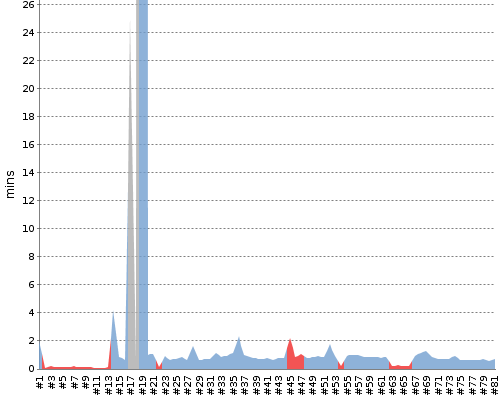
\includegraphics[bb=0 0 500 400, scale = 0.6]{build-trend.png}
\caption{Build trend summary. Vast majority of builds are well under 10 minutes. Outlying values were caused by a network outage.}
\end{figure}

\subsection{Measuring Test Coverage}

Since we did not adopt a TDD approach from the very beginning, it was important to obtain an overview of the parts of the code that required testing. Starting with iteration 5 we have used Cobertura,  an open source tool which provides neat test coverage reports for Java programs.

To facilitate report generation, a single ant task has been set up to compile the code with the debug info (vital for Cobertura to indicate line numbers and measure coverage), run all the tests (unit, acceptance, integration) and generate human readable reports which provide an indication of the current test coverage as well as branch coverage and complexity measures.

The coverage reports enabled us to identify lines which were not touched by tests. This was usually fixed by writting another test to cover the specific path, but it could also have been the case that the functionality was actually never required, in which case it was completely removed. Again this illustrates how tests have been used to ensure we are running a healthy codebase.

Branch coverage indicates when tests do not cover particular cases and has proven useful with regards to particularly tricky conditionals.

Cobertura also generates cyclomatic complexity values for each class/package, measuring the number of independent paths through the control flow graph of the code. Since it has been shown that high values are usually an indication of error prone code[2] this measurement is used to check code sanity.

\begin{figure}[ht]
\centering
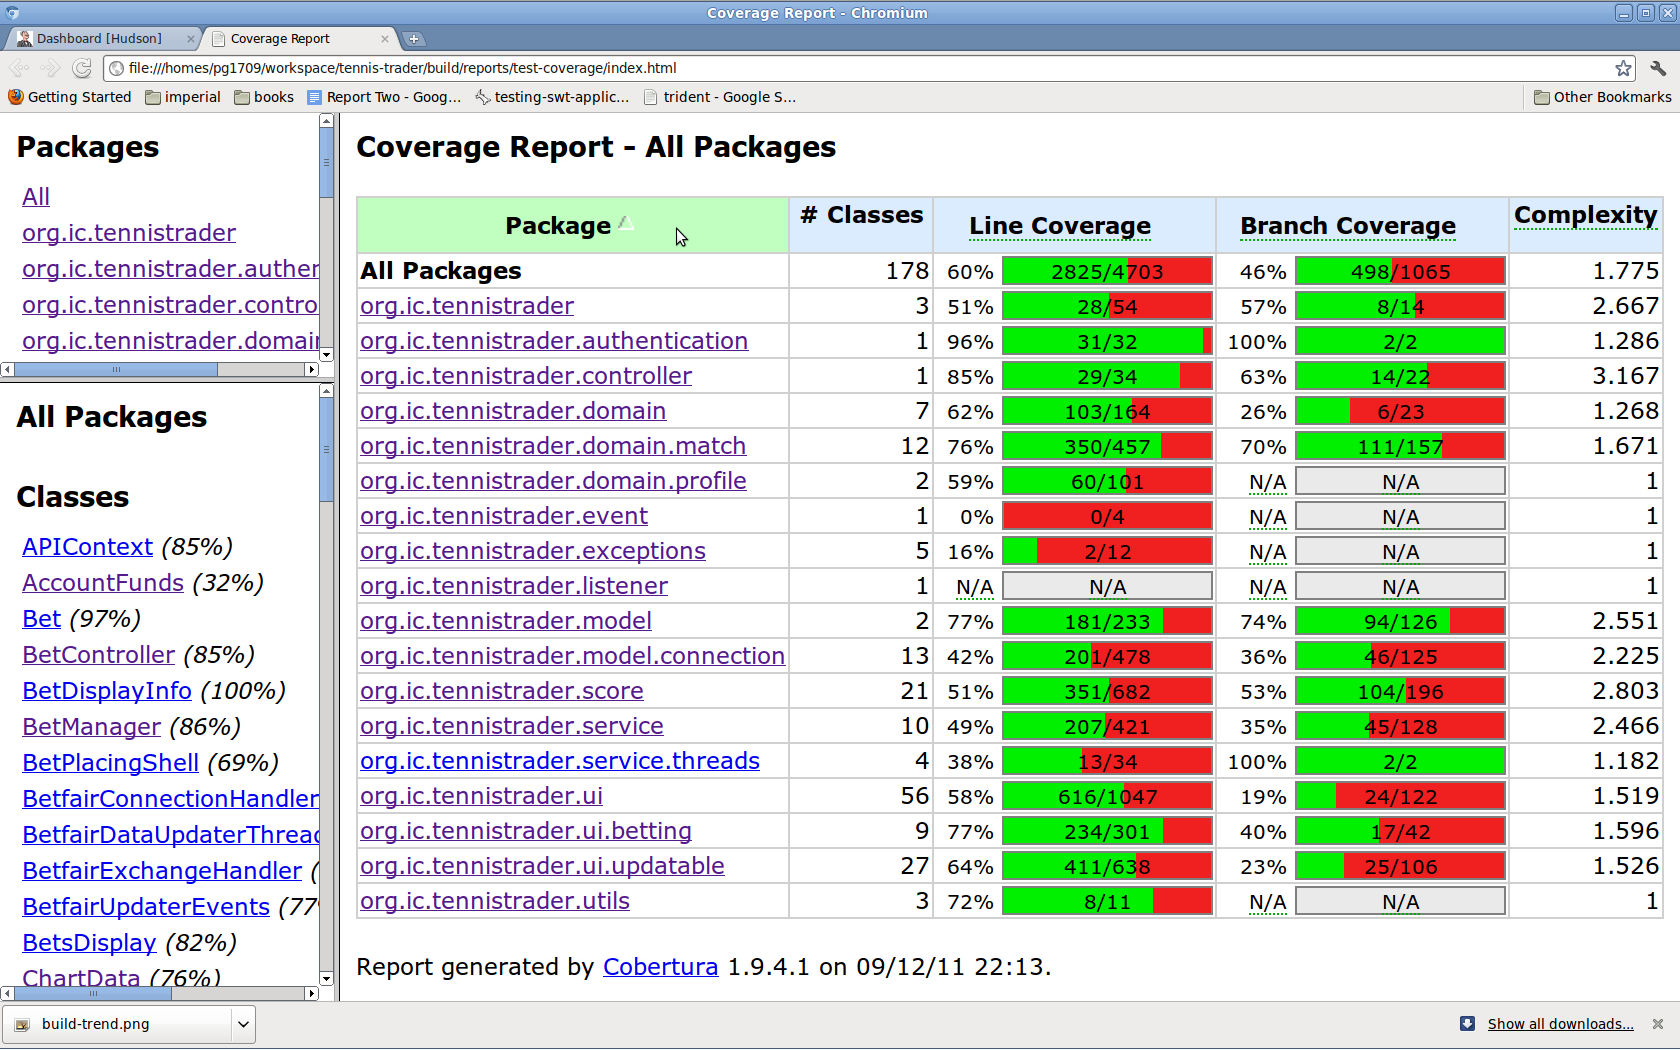
\includegraphics[bb=0 0 1680 1050, scale = 0.2]{coverage.png}
\caption{Coverage report generated by Cobertura indicates test coverage at package level, branch coverage an cyclomtic complexity.}
\end{figure}



\begin{figure}[ht]
\centering
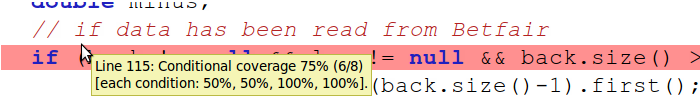
\includegraphics[bb=0 0 700 100, scale = 0.49]{branch.png}
\caption{Branch coverage indicates specific condition coverage.}
\end{figure}

\subsection{Code Quality Measures}

We have used PMD to generate code quality reports. Additionally we have researched and are looking forward to using FindBugs - a tool which identifies bugs (such as NPEs and potential out of bounds accesses) for Java code.

\begin{figure}[ht]
\centering
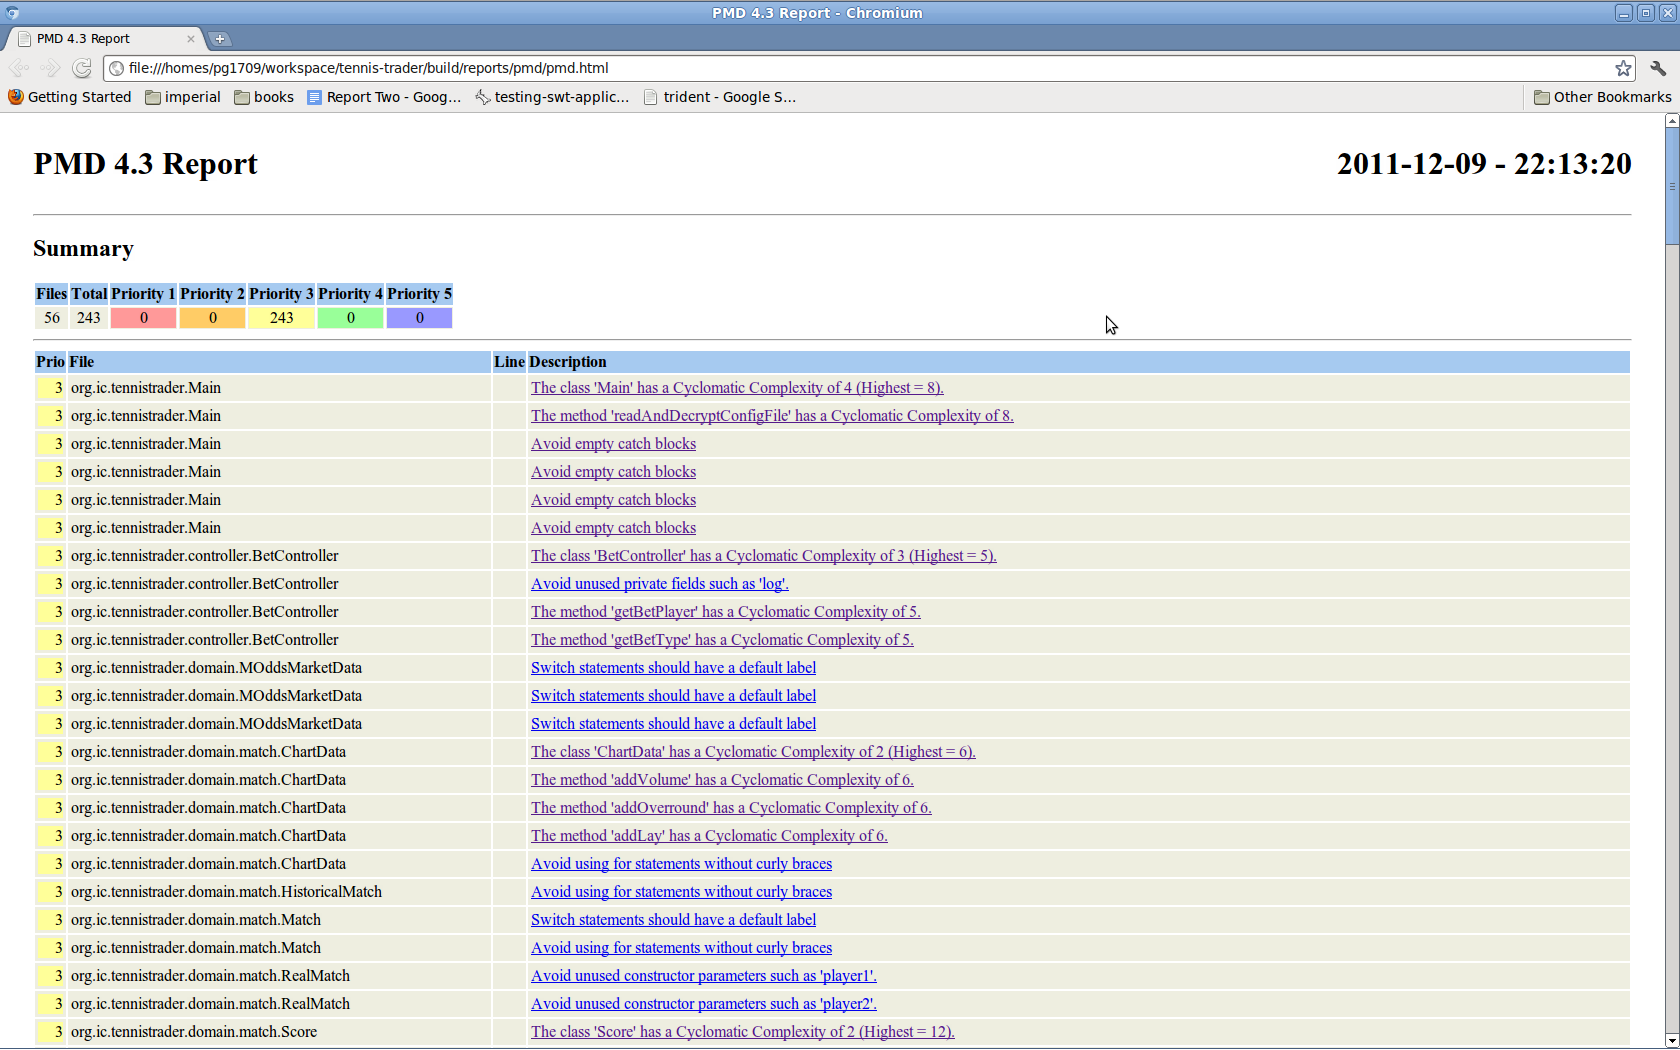
\includegraphics[bb=0 0 1680 1050, scale = 0.2]{pmd.png}
\caption{PMD reports indicate potential quality issues. The tool can be configured to signal a host of potential issues (such as ...).}
\end{figure}

\subsection{Logging}
**
We have used logging to aid the development process (especially debugging).
**
\subsection{Test Guided Design}
**
Refactoring

Used extract superclass, pull up (for tests), extract class
**
\subsection{Portions of code base tested}

All core components of the proTrade application have clear distinctions between back/front ends, local/enternal data, and internal state/state handler-updater. The modular design is in direct relation with testing methodologies chosen, with unit tests validating the former ends and functional/acceptance tests testing the latter. On top, integration tests are used to reproduce and analyse behaviour of specific GUI or data fetching/updating libraries that are used in conjunction with local features. A functional overview of the applications's code base and features together with their tests is given below:

\begin{itemize}
\renewcommand{\labelitemi}{$\bullet$}
\item Authentication: Encrypt/decrypt functions for storing and accessing the login credentials are unit tested, while the interface (LoginShell) is acceptance tested (as detailed in section 2.2).
\item Controller: The bet controller, built upon relevant back/lay buttons and their associated bet placing functionality, is tested for correct bet types and player recognition.
\item Domain: Local functionality of populating/retrieving the chart widget with market data is unit tested in 'ChartDataTest'. Specific tests for other domain classes have not been designed, since these are plain java objects, with no logic implementation. However, their functions are tested when these objects are used in other unit-tests.
\item Domain/match: Special unit-tests have been designed to check how the score of a match is updated and handled.
\item Model and Model/connection: The implementation and logic of virtual betting (including the internal state representation of the market and matched/unmatched bets) are unit tested, while the global and exchange connections to Betfair API (that normally update the internal state) are validated via integration tests.     
\item Score: Front end 'PredictionGui' controller is functionally tested, whereas specific unit tests are written for back-end components such as statistics fetching and parsing or the 'PredictionCalculator' model. 
\item Service: Since this package models the back end receiver for various incoming data, state updating is unit tested.
\item UI and UI/Betting: Acceptance and testing of all front-end GUI interfaces.
\item UI/Updatable: Acceptance and integration testing on dynamical GUI elements driven by user input or data updates.
\end{itemize}

\begin{figure}[ht]
\begin{center}$
\begin{array}{ccc}
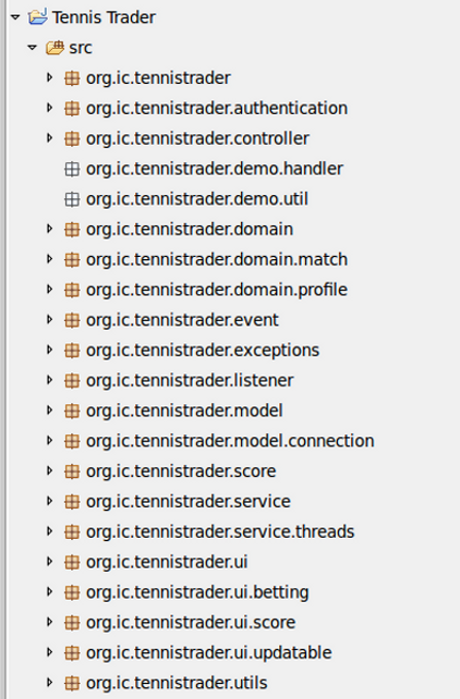
\includegraphics[bb=0 0 499 700, scale = 0.25]{project.png} &
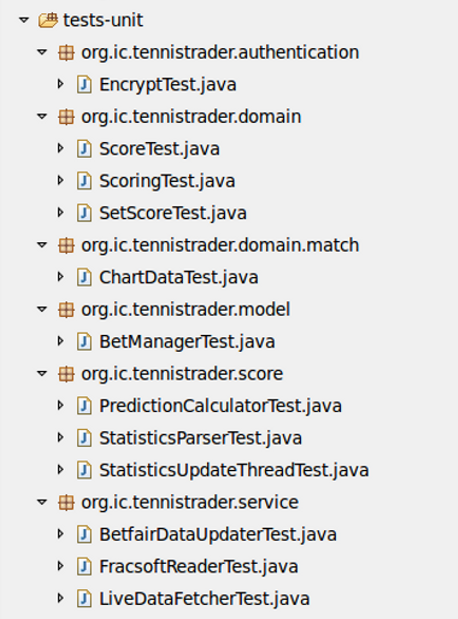
\includegraphics[bb=0 0 499 700, scale = 0.25]{tests-unit.png} &
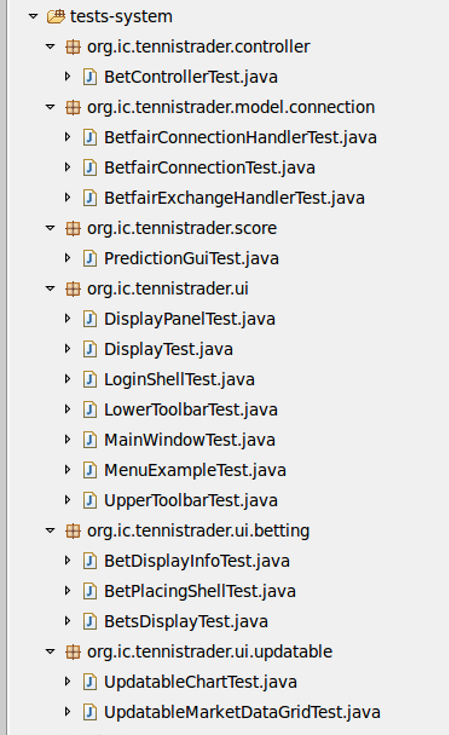
\includegraphics[bb=0 0 499 700, scale = 0.25]{tests-system.png} 
\end{array}$
\end{center}
\caption{Left - Project hierarchy with included packages. Center - Unit tests for local functionality/model based classes/packages. Right - System tests for controller/UI oriented classes/packages}
\end{figure}

\subsection{Bugs/problems revealed by testing}

Apart from validating design, testing has revealed hidden bugs in various components of the system. 

Unit tests have invalidated a first encoding of the scoring system for the prediction calculator, when translating between traditional tennis point scores and an incremental representation.

Also, they have identified a missing condition when registering events whose market data should constantly updated by connecting to the Betfair API, which resulted in some events being introduced twice.

Furthermore, they have revealed some overlooked considerations in recursive state passing when computing a set prediction based on a Markov chain model, which led to wrong set winning probability estimates. 


\section{General Validation}

General Validation: to decribe any other methods you may have used to validate your executable deliverable; the following list is only suggestive but should give you an idea of what things you could do:

\subsection{User interface design validation}

The user interface of our application has been designed with a view towards obtaining a final product which achieves the following goals: it is visually eye-pleasing, it is simple to use, it minimizes the effort it takes for users to accomplish their work/wish/..
To the purpose of validating our user interface design, feedback has been collected from a number of different persons with or without experience in using trading applications.

\subsubsection{Feedback from Experienced Users}

Firstly, we have had constant feedback from our supervisor, who is familair with the game of tennis and tennis betting and who understands the needs of a professional trader. He has guided us through the process and has pointed out a number of possible UI improvements along the way (such as positioning different components, displaying different data on the graph), which we have accomplished.

Secondly, we have had meetings with PhD students, who are themselves developing trading applications. They gave us valuable feedback regarding market information display and the best way to present it to a specialized user. Hence, our initial interface has been adapted to accommodate their suggestions (e.g. displaying some additional market statistics) - supported by our supervisor.

Finally, to collect feedback from other points of view as well, our supervisor arranged for us to meet the head of research of Betfair. He has approved(?) of our application's general interface and pointed out a few possible issues (such as synchronizing all the playback data), which are now fixed(?).

\subsubsection{Feedback from Unexperienced users}

To test how easy it is for users to understand the information presented by our application and how ''natural'' to find the required functionalities, we have collected feedback from a few colleagues, without previous experience with tennis trading applications. (??? - what did they say?)

Overall, the interface of our application has been validated by the users, with some improvement suggestions which we have considered and implemented.


\subsection{Code Review}

We also used a review mechanism in which, normally, code has been inspected by at least two team members.


During the implementation process we often employed pair programming but also other lightweight code review mechanisms[3], particularly over-the shoulder and tool-assisted code review (e.g. based on PMD suggestions).
The decision to adopt lightweight code review mechanisms was based on evidence presented in [4], which suggests that this type of review can be as effective as a more formal one, but easier to implement.

This helped improve the overall quality of the software and minimize the number of bugs early on in the development process.
The whole source code is accessible to every member of the group and where appropriate and necessary, the code is reviewed by other members who don’t work on that specific widget or feature. 

Where a bug is found or refactoring is needed, usually an issue is raised on GitHub with the suggestion to solve that specific problem.

As this is done on a regular basis, we have agreed from the beginning to comment the code as much as possible and to use coding standars

\subsection{Stress testing}

At the moment, no stress testing tools are used. Our group left this as the last stage of our development process, as this may be more beneficial once we have all the features implemented.
However we have conducted a `manual` stress testing.

An abnormal condition or a stressing condition for our application is when a user tries to view and trade several matches/markets at the same time. This is done by opening more than one tab, where each tab displays the match/market.

We have observed that when we open a single match/market the physical memory consumed by the application is 1.5 GB and once we open more matches/markets this figure increases even more reaching 2GB when 3 tabs are opened. This enforced us to raise an issue with high importance and it is an on-going process where we try to identify any memory leaks, to analyse if we store any redundant/unused data and any other ways to reduce this figure. We understand that this is a major issue as an average computer has 3-4 GB of physical memory and we aim to solve the problem by the end of the project.

We are using Standard Widget Toolkit (SWT) to develop our graphical user interface and since the native OS widgets creatde by it cannot be garbage collected, a special attention is paid to creating and disposing the components, in order to avoid any memory leaks.

Our application requires a lot of data to be stored and presented to a user in a special way, one of the aims of the group is to have an efficient memory management, as this will lead to a better responsiveness of the application which is vital for traders.

Our application does not consume a lot of CPU power as our computations are negligible except to a few data statistical/technical analysis of data which is vital for traders, but we haven’t observed a heavy CPU usage even with many concurrent markets/matches ope

\subsection{Did you test the GUIs of your software?}

We mentioned above that we are using the SWTBot API to test our widget and unfortunately because of its limitations we haven’t yet identified ways to test the functions of the specific components such as the context menu (pop u) or a progress bar. However we realise that this is very important to test before realising the application. One of the most important tools for traders is the chart where they can view the flow of a market and we must implement it very efficient and to make sure that the graphical part of it is working properly. We have implemented a context menu on the chart, where the user may select different types of analysis to be shown and as we can’t test the context menu we are not sure of the potential behaviour of the application in certain conditions.


\section{Managerial Documentation}
\label{sec-group}

This section provides a formal account of group management and activities.

\subsection{Collaboration Tools}

Throughout the project various collaboration tools were used that would help in cooperation for successful product delivery.

\subsubsection{Git}

Use of Git significantly improved the quality of the work produced by the team, as it provided not only a shared code base with version control, but also a good picture of the current state of the project. Moreover, it encouraged team members to use ``Commit Early, Commit Often'' paradigm, as many postponed commits tend to result in a large number of merge conflicts. This increase in the commit frequency simplified error tracking and resolving.

\subsubsection{Github repository}

For the purpose of efficient collaboration, a private Github repository was created, providing the team with a wide range of features. First of all, the team used issues that could be tracked and assigned to specific group members. These had comment threads linked to them, simplifying communication and giving an ability to have almost instant feedback on the solution. Moreover, use of issues dramatically increased the team's efficiency, for example, whenever there was a new issue added to the back log, all teammates were notified, and once one of them had finished work on his or her piece, that member could then start thinking on another problem. Furthermore, the Github repository provided the ability to split issues into different milestones, consequently giving a better sense of direction to everyone in the group, which in turn increased the level of cooperation between team members.

\subsubsection{Google Docs}

Another set of collaboration tools that proved to be useful was Google Docs. This platform allowed the whole group to exchange information by creating shared documents. The team primarily used it to write meetings agendas, keep logs of the work done via spreadsheets and set global objectives for particular iterations. The use of google docs also simplified report editing by providing support for concurrent editing and instant feedback (via the ``comment'' feature).

\subsubsection{Dropbox}

In order to manage access to larger files, Dropbox accounts were created which allowed team to share data related to tennis (e.g. match videos), sports trading, documentation for the Betfair API etc.

\subsubsection{Email, Skype and IM}

To establish a concrete communication channel throughout the project group, it was essential to have a good medium that everyone would have an access to. Therefore, the group's choice has fallen on electronic mail and messaging services. Emails provided good updates for the whole team and simplified the process of making proposals and raising issues that needed consideration of all team members. Skype and IM services, in turn, made it easier for several group members to work on specific issues and provided an excellent medium for knowledge exchange.

\subsection{Management Policies}

Management Policy is a documented set of rules, constraints, standards and guidelines that apply to the decision making and determination of an action, for both present and future state, and for a specific area of interest or concern that relates directly to Software Development, based on a set of given inputs, conditions or state.

\subsubsection{Code Change Policy}

In order to deliver a successful project, the team had to have a strict set of policies addressing code change. In our case, at first, the continuous integration server was used to keep track of how many tests are covered and which parts need more development. On top of that it also provided a good analitical base for issue resolving, for example, in case a commit broke the build, it was relatively easy to track it down.

However, in the last 10 builds our project group experienced 5 breaks, thus, the team decided to change to a more stable code quality control system - branching. The idea behind it is to have to different branches: master (dev) for development purposes and stable (release) for a latest stable version, thoroughly tested and agreed with every team member. Consequently, while master branch is open for commits from everyone inside the project group, stable version is only accessible to the team leader. This way team always has a stable version to fall back to at the end of every iteration.

\subsubsection{Validation Policy}

Before implementing the branching system the team did not have a set of rules for commits, resulting in numerous build breaks for continuous integration server. The team agreed that this was not an efficient way of code quality control, thus, new rules for code commited were enforced. 

From now on, any change to the code in the Release was to be overviewed by two other team members, giving the group necessary level of code validation and quality control. As a result of this policy, team gained experience in code review and improved technical expertise by the information exchange through problem solving.

\subsection{Knowledge Transfer}

Knowledge transfer within the project group was managed by the several techniques, specific to agile software development paradigm. In this particular case, the team made use of issues with comment threads to pass the obtained information on the solution. Furthermore, stand-up meetings were arranged to help individual members. During these meetings teammates would explain the nature of obstacles met, so that others could support them with background knowledge on the subject. Finally, documents passed through dropbox and google docs contained information on software packages used, to help group members obtain more explicit knowledge on the topic.

All in all, efficient management of knowledge transfer within the team required a constant stream of feedback from other members upon the work produced. This significantly improved the transfer of tacit knowledge within the group, consequently helping to overcome most of the obstacles in development.

\subsection{Materials}

Below are the tables of the group meetings including dates, format and which members attended, hours spent per week on which tasks or activities by each member on the project and the Log-book.

\begin{thebibliography}{9}
\bibitem{bk-testing}
  Steeve Freeman, Nat Pryce,
  \emph{Growing Object-Oriented Software, Guided by Tests}, Addison-Wesley 2010

\bibitem{web-cyccom}
  Robert Chatley's course on Software Engineering Methods
  \url{http://en.wikipedia.org/wiki/Cyclomatic_complexity},
  Imperial College London

\bibitem{bk-aglsam}
  Jonathan Rasmusson,
  \emph{The Agile Samurai},
  Pragmatic Bookshelf,
  October 2010.

\bibitem{bk-aglflh}
  Jeff Langr and Tim Ottinger,
  \emph{Agile in a Flash},
  Pragmatic Bookshelf, 
  January 2011.

\bibitem{web-rbc}
  Robert Chatley's course on Software Engineering Methods
  \url{http://www.doc.ic.ac.uk/~rbc/302/},
  Imperial College London

\bibitem{site-fracsoft}
  Site of Fracsoft, authors of Fracsoft Data Viewer
  \url{http://www.fracsoft.com}

\bibitem{site-betangel}
  Site of BetAngel
  \url{http://www.betangel.com}
  
\bibitem{wiki-swt}
  SWT - Wikipedia
  \url{http://en.wikipedia.org/wiki/Standard_Widget_Toolkit}

\end{thebibliography}

\end{document}
